\documentclass[fontsize=11pt]{scrartcl} % A4 paper and 11pt 
\usepackage[T1]{fontenc}
\usepackage[font=small]{caption}
\usepackage{wrapfig}
\usepackage{sectsty} % Allows customizing section commands
\usepackage[margin=1in]{geometry}
\usepackage[procnames]{listings}
\usepackage{color}
\usepackage{graphicx, subcaption}
\usepackage{algorithm2e}
\usepackage{titlesec}
\usepackage[svgnames]{xcolor} 
\allsectionsfont{\centering \normalfont\scshape} % Make all sections centered, the default font and small caps
%\usepackage{natbib} 
\usepackage[breaklinks,hidelinks]{hyperref}
\usepackage[ margin=.2cm]{caption}
\usepackage{fancyhdr} % Custom headers and footers
\pagestyle{fancyplain} % Makes all pages in the document conform to the custom headers and footers
\fancyhead{} % No page header - if you want one, create it in the same way as the footers below
\fancyfoot[L]{} % Empty left footer
\fancyfoot[C]{} % Empty center footer
\fancyfoot[R]{\thepage} % Page numbering for right footer
\renewcommand{\headrulewidth}{0pt} % Remove header underlines
\renewcommand{\footrulewidth}{0pt} % Remove footer underlines
\setlength{\headheight}{10.6pt} % Customize the height of the header
\setlength\parindent{0pt} 
\setlength{\parskip}{1em}

\newcommand{\horrule}[1]{\rule{\linewidth}{#1}} % Create horizontal rule command with 1 argument of height

\graphicspath{{../figures/}}
\DeclareGraphicsExtensions{.png, .jpg}

\usepackage{booktabs} % Top and bottom rules for table
\usepackage[font=small,labelfont=bf, skip=0pt]{caption} % Required for specifying captions to tables and figures
\usepackage{amsfonts, amsmath, amsthm, amssymb} % For math fonts, symbols and environments
\usepackage{wrapfig} % Allows wrapping text around tables and figures
\usepackage{titlesec}
 
 
\title{	
	\normalfont \normalsize 
	\textsc{North Carolina State University} \\ [5pt] % Your university, school and/or department name(s)
	\horrule{0.5pt} \\[0.4cm] % Thin top horizontal rule
	\huge An Online Algorithm For A Low Cost Real-Time Sensor-Based Fenceline Leak Detection System\\ % The assignment title
	\horrule{2pt} \\[0.5cm] % Thick bottom horizontal rule
}
\author{Halley Brantley, Yichen Si, \& Dendi Suhubdy} % Your name
\date{\normalsize December 7, 2015} % Today's date or a custom date
 
\begin{document}
\definecolor{keywords}{RGB}{255,0,90}
\definecolor{comments}{RGB}{0,0,113}
\definecolor{red}{RGB}{160,0,0}
\definecolor{green}{RGB}{0,150,0}

\maketitle

\section{Introduction}
Benzene is an air pollutant and carcinogen that is regulated by the U.S. Environmental Protection Agency (EPA) and often emitted by petroleum refineries as a result of leaking equipment and wastewater treatment \cite{fencelinerule}. Cost-effective and real-time methods for monitoring hazardous air pollutants emitted from industrial facilities could lead to faster leak detection, repair, and reduced emissions. One monitoring method currently under development by the EPA's Office of Research and Development is the SEnsor NeTwork INtelligent Emission Locator (SENTINEL) that combines time-resolved measurements and inverse models of various forms to improve source understanding on a variety of spatial scales \cite{wan2015}. We present here an algorithm for locating the source of emissions using 1 Hz benzene and wind sensors.  
\vspace{10pt}

\section{Data Description}

\begin{figure}[h!]
	\begin{subfigure}[b]{0.43\textwidth}
		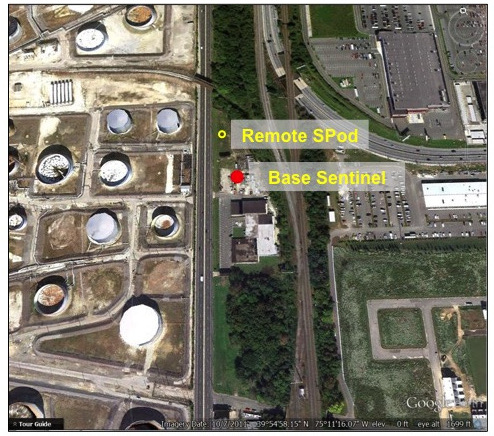
\includegraphics[width=\linewidth]{Slide11}
	\end{subfigure}
	\begin{subfigure}[b]{0.5\textwidth}
		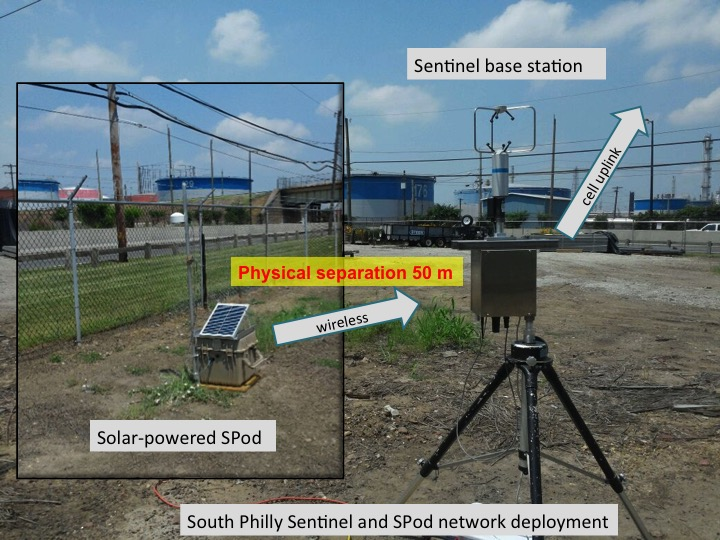
\includegraphics[width=\linewidth]{Slide12}	
	\end{subfigure}	
	\caption{Sensor location and equipment.}
\end{figure}

The sensor system used to collect the measurements in this study consisted of two units: a solar-powered "sensor pod" (SPod) controlled by a low cost and low power Arduino UNO computer and a wired SENTINEL base station containing an Intel Atom\textsuperscript{TM} computer (Santa Clara, CA, USA) and a model 81000V 3-D Ultrasonic Anemometer (R.M. Young, Inc., Traverse City, MI, USA) that provides 1 Hz wind measurements. Both systems log time-synchronized 1 Hz data from a custom EPA-developed sensor boards containing a 10.6 eV passive photoionization detectors (PIDs) (blue label piD-TECH \textsuperscript{\textregistered}, Baseline-Mocon Inc. Lyons, CO, USA) used to detect benzene. \cite{wan2015} 
\par The sensor system was deployed near a refinery in South Philadelphia from July, 2014 through February, 2015. PID sensor response and stability are affected by temperature, humidity, lamp deposition and other variables resulting in unwanted baseline drift that complicates data analysis.	The PID sensor output ranges from 0.2 to 5 volts resulting in both left and right censoring. Two days of 1 s measurements are shown in Fig 2.  	
 

\begin{figure}[h!]
	\begin{subfigure}[b]{\textwidth}
	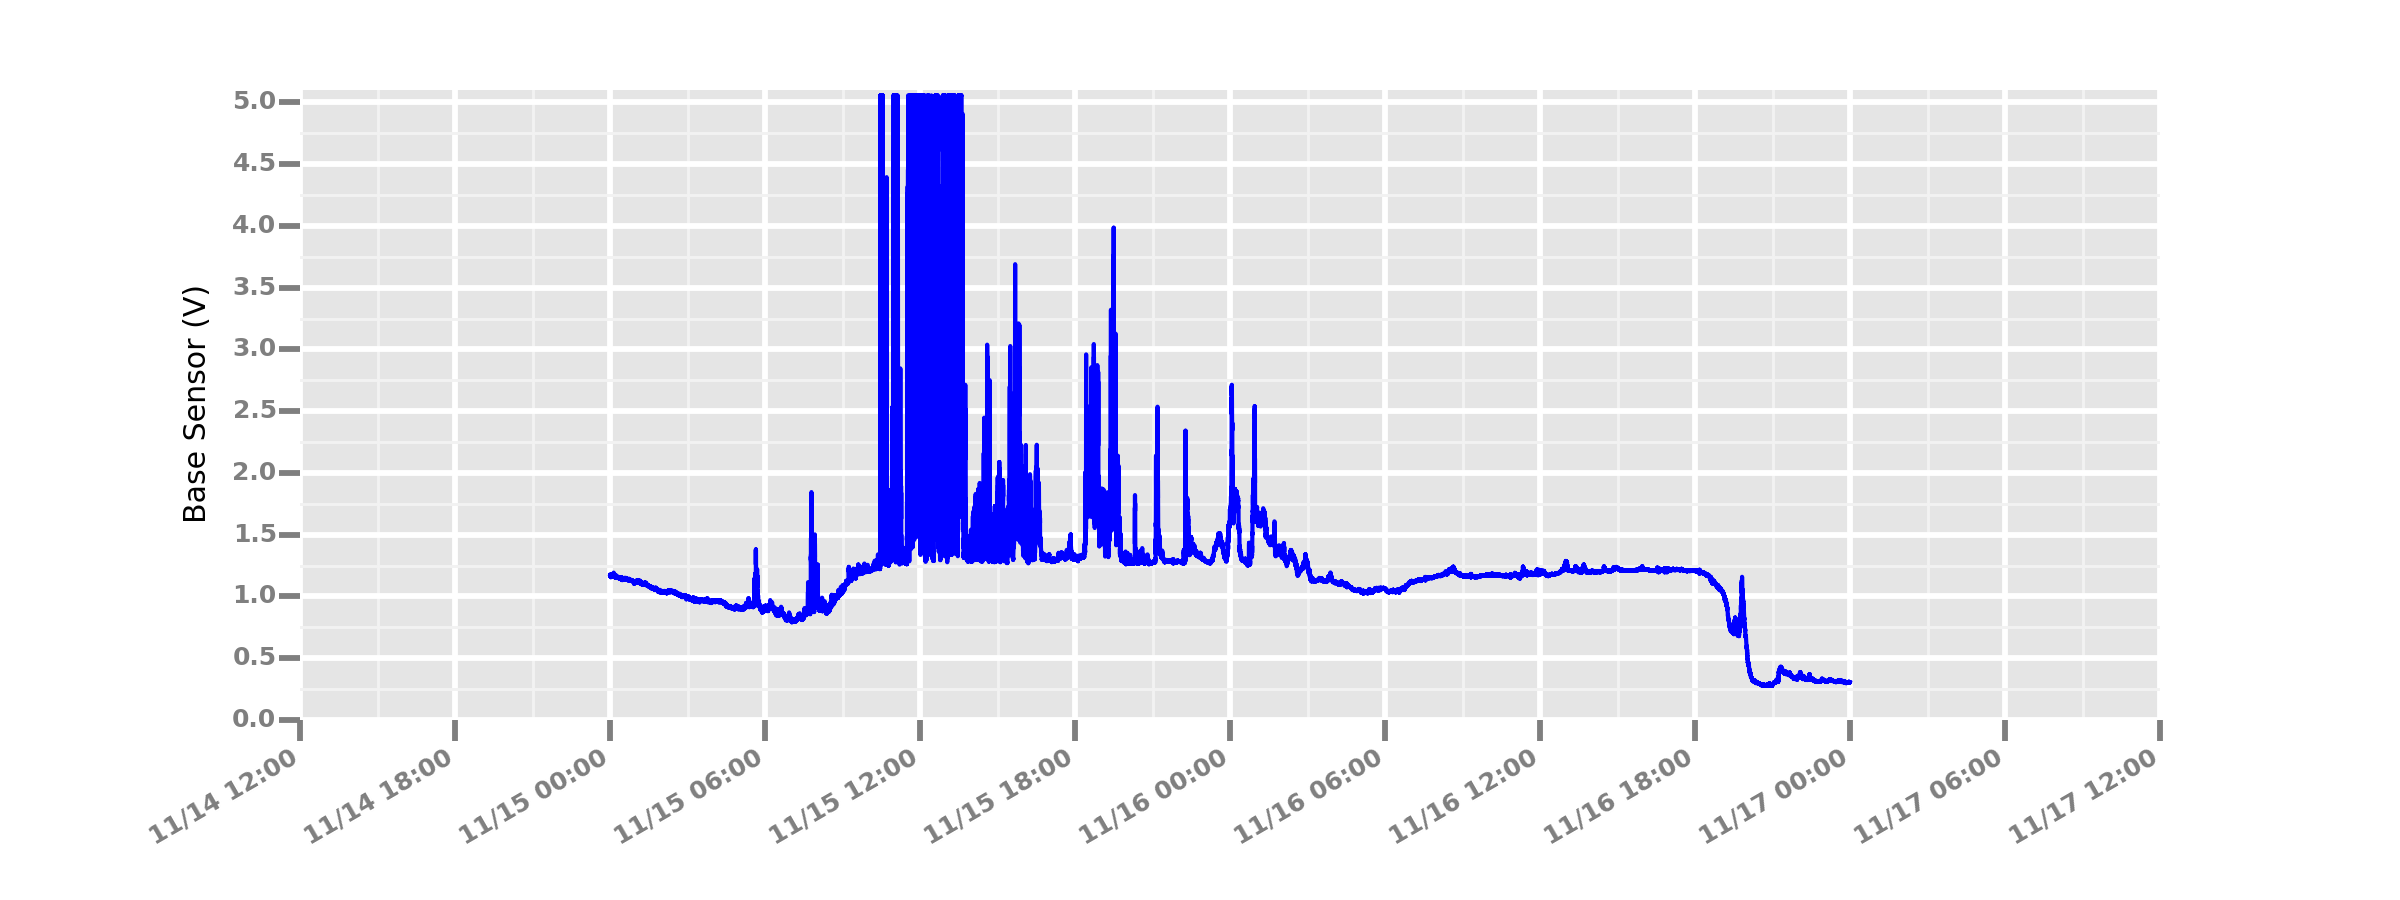
\includegraphics[width=\linewidth]{Base}
	\captionof{figure}{Base Sensor Signal}
	\end{subfigure}
	\begin{subfigure}[b]{\textwidth}
	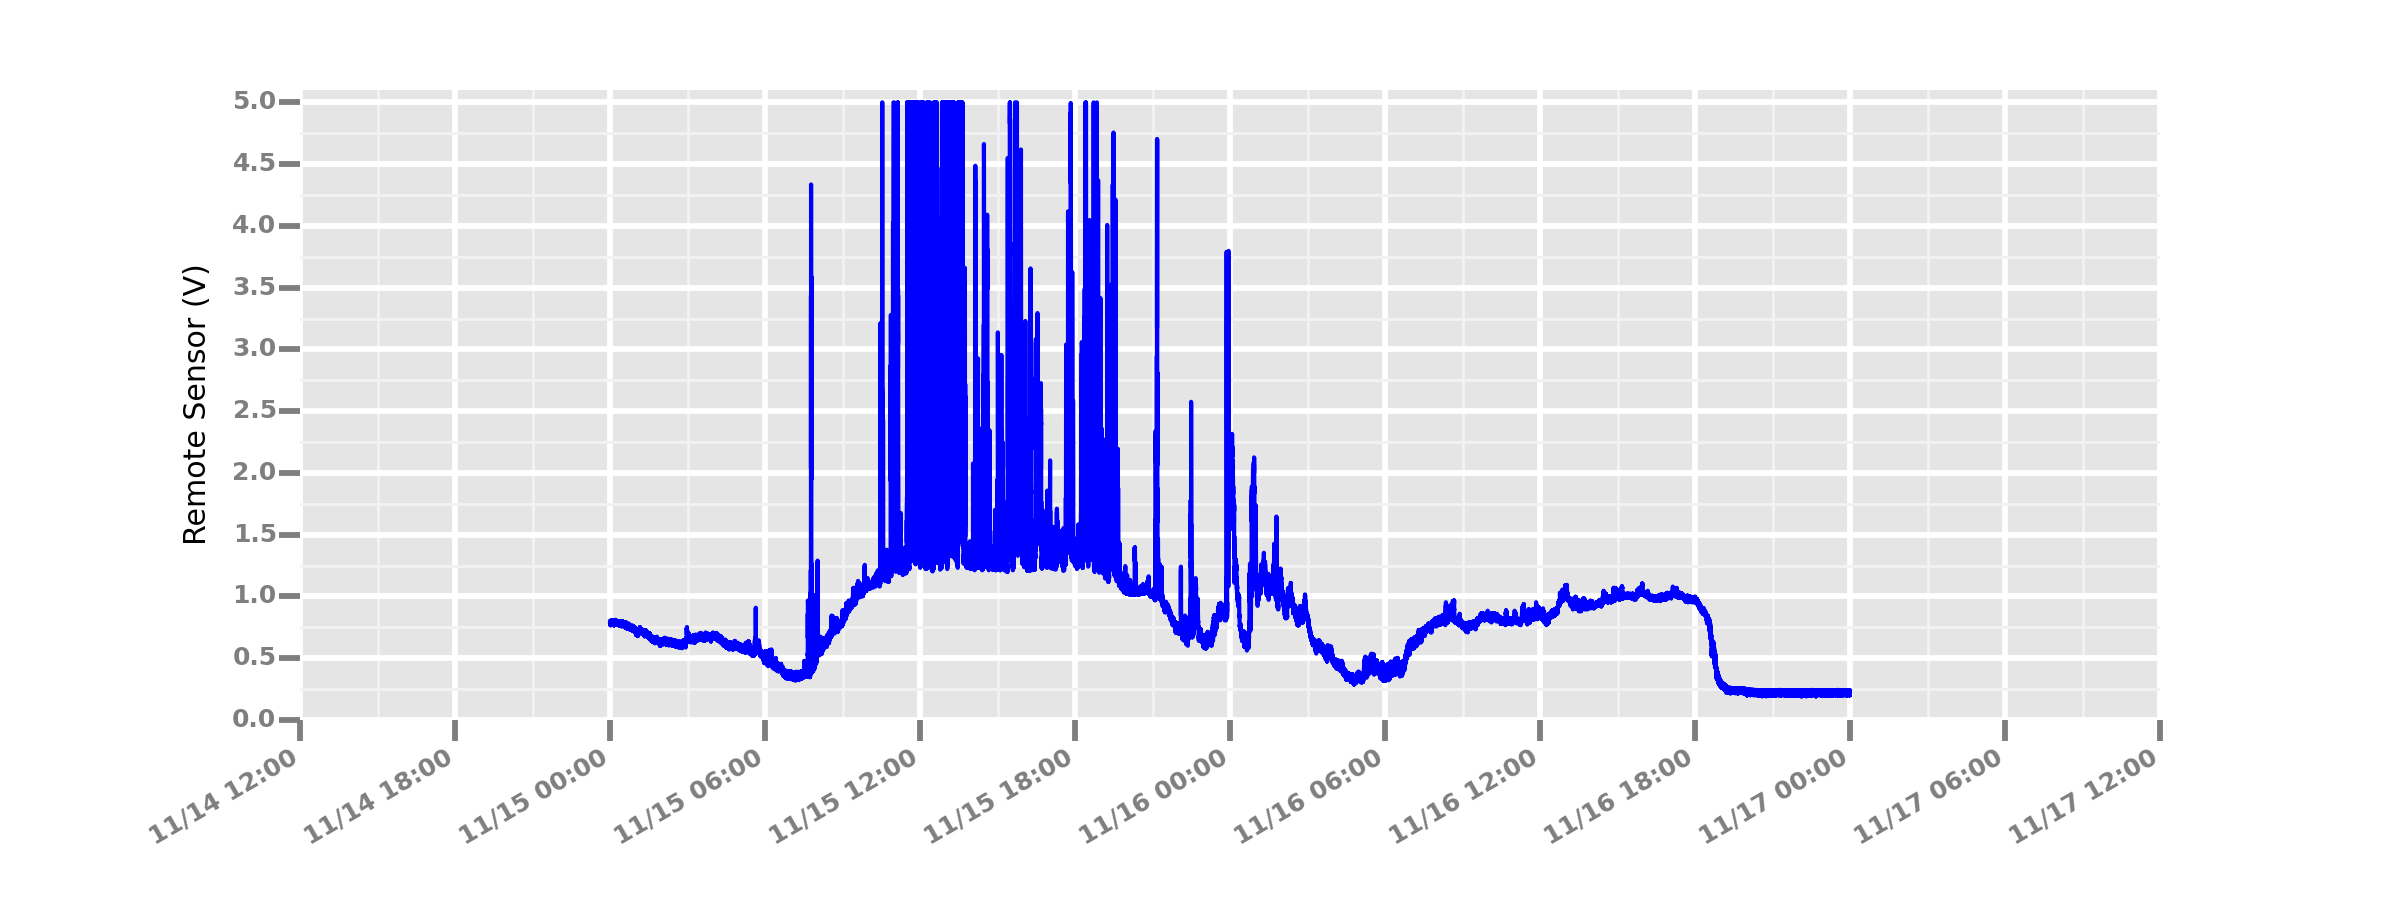
\includegraphics[width=\linewidth]{Remote}
	\captionof{figure}{SPod Sensor Signal}	
	\end{subfigure}
	\caption{Measurement example.}
\end{figure}

\section{Simulated Data}

Concentrations for 4 hours were simulated for each of the sensors using the Quick Urban and Industrial Complex (QUIC) Dispersion Modeling System \cite{QUIC}.  Inputs to the modeling system included wind measurements averaged to 5 minute intervals from July 5, 2014 from 12:00-16:00. A logarithmic wind profile was used and a single source location was chosen (Fig 3).  For the simulation, 1728000 particles were used with a 2 sec time step and a concentration averaging time of 20 sec.  
\par

\begin{figure}[h!]
	\centering
	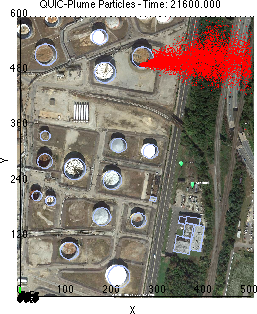
\includegraphics[width = 0.5\linewidth]{QUIC_fig}
	\caption{Location of source for QUIC model.}
\end{figure}

Further analysis was conducted in Python 2.7.9 \cite{python} using the SciPy 0.16.1 and NumPy 1.10.2rc1 libraries \cite{scipy}. The QUIC concentrations were output at 20 sec and up-sampled in Python to 1 sec by repeating the previous value (Fig 4a). Each hour of the stochastic baseline was simulated as 1D Brownian bridge with each 1 s step drawn from a $\mathcal{N}(0, 1/3600)$.

An offset of 1.5 was added to the simulated baseline, to imitate the measured values. After the simulated baseline and concentration were added, values above above 5 were censored to 5 and values below 0.25 were replaced with random draws from a $\mathcal{N}(0.25, 0.05)$.  

\newpage

\begin{figure}[h!]
\begin{subfigure}[b]{\textwidth}			
	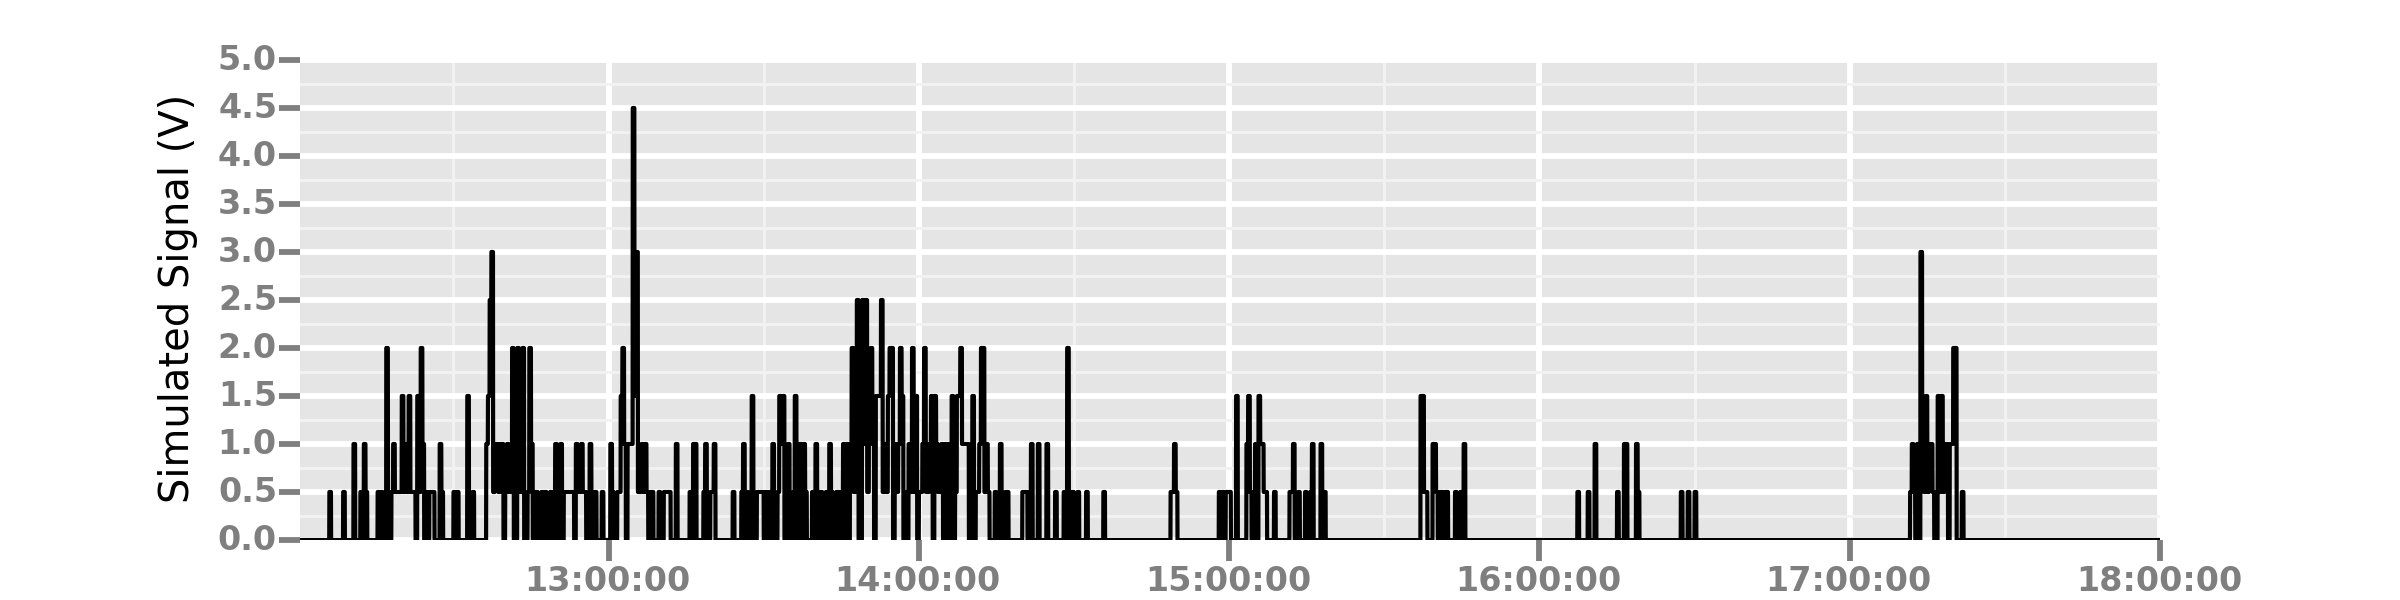
\includegraphics[width=\linewidth]{BaseSim}
	\captionof{figure}{Base Sensor Simulated Concentration from QUIC}
\end{subfigure}
\begin{subfigure}[b]{\textwidth}
	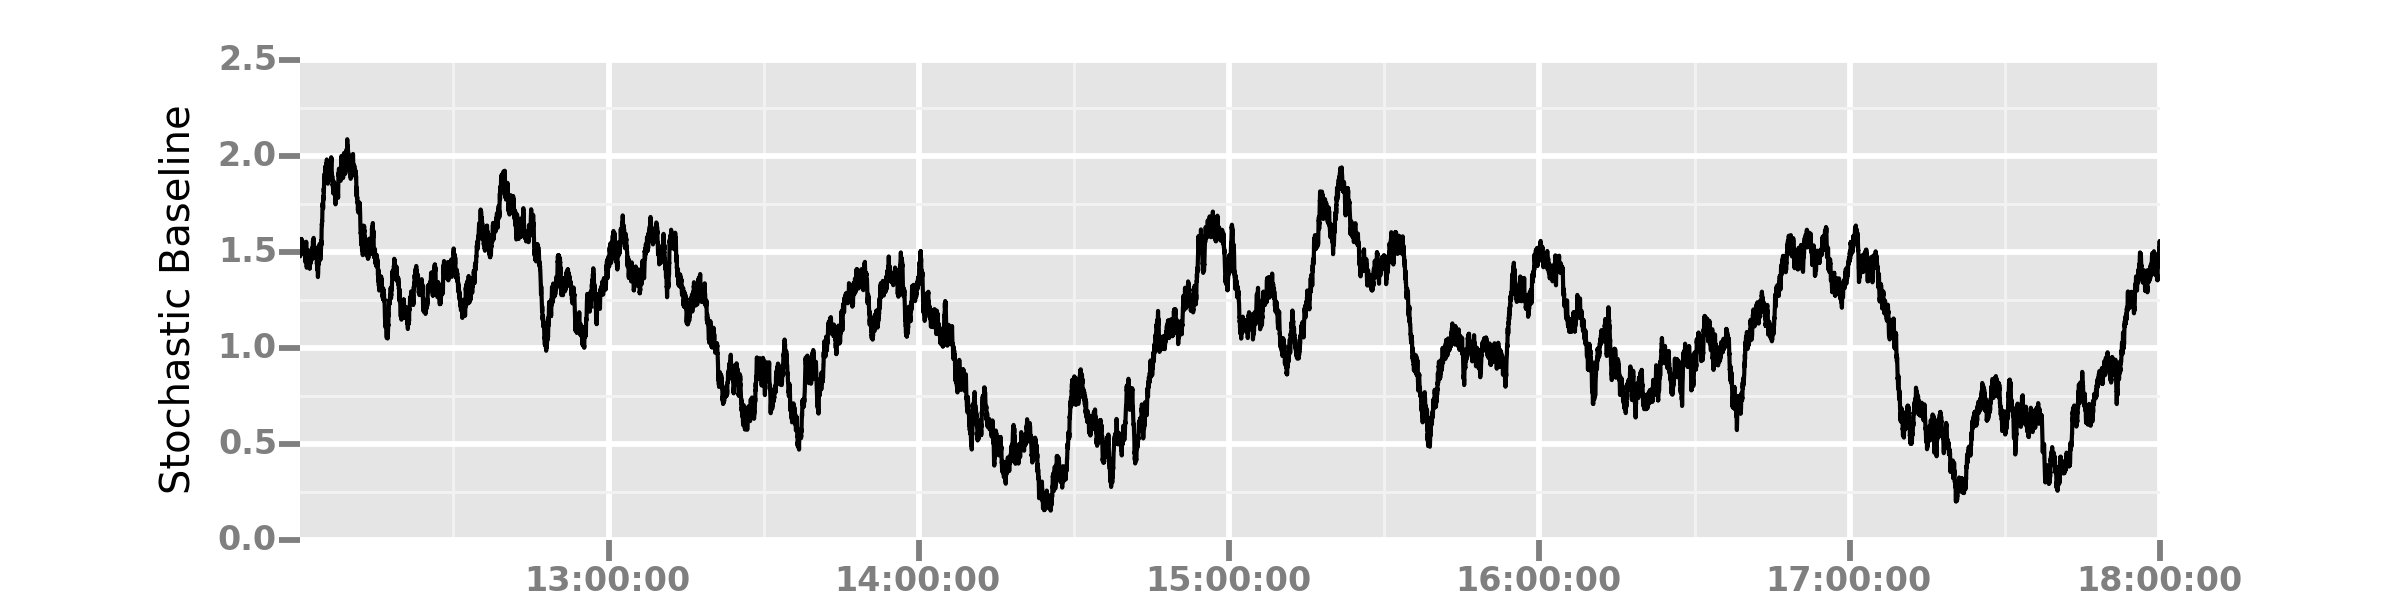
\includegraphics[width=\linewidth]{BaseRand}
	\captionof{figure}{Base Sensor Simulated Stochastic Baseline}
\end{subfigure}
\begin{subfigure}[b]{\textwidth}
	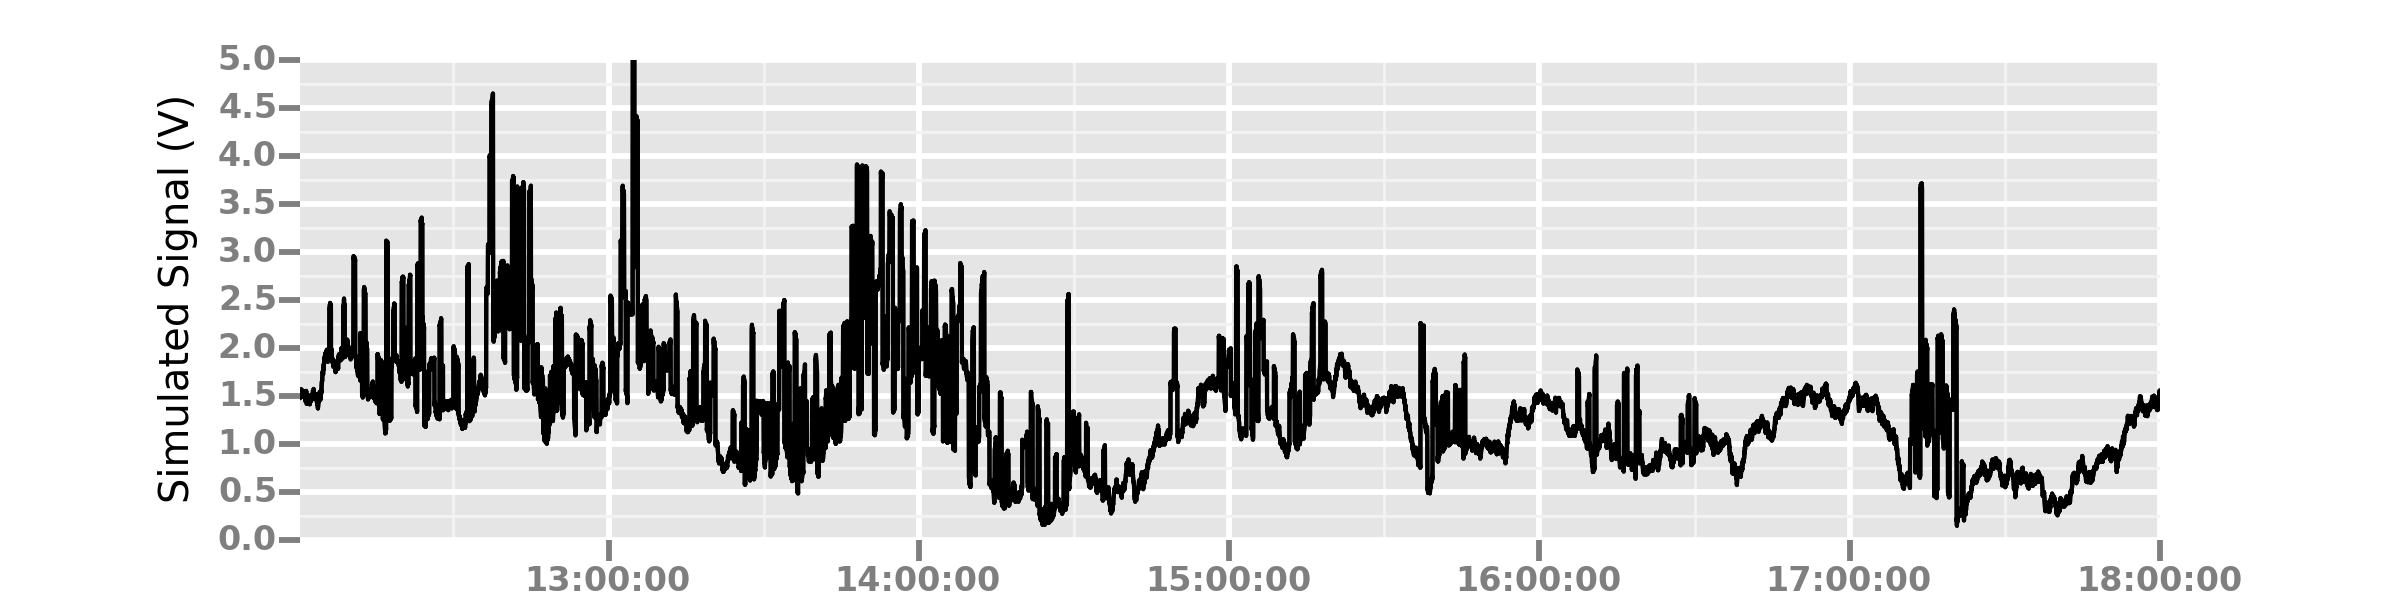
\includegraphics[width=\linewidth]{BaseTotal}
	\captionof{figure}{Base Sensor Simulated Data}
\end{subfigure}
\begin{subfigure}[b]{\textwidth}
	\includegraphics[width=\linewidth]{RemoteTotal}
	\captionof{figure}{SPod Sensor Simulated Data}	
\end{subfigure}
\caption{Simulated Data.}
\end{figure}

%------------------------------------------------
\newpage

\section{Algorithm Description}
Two different methods of separating the concentration signal from the baseline drift and the noise were investigated and applied to 3 hour slices of the simulated data. The methods were also tested using 1 and 2 hour segments and produced similar results. The outline of the algorithm is given in Algorithm 1. 

%% adding algorithm steps in latex
\begin{algorithm}[H]
	\KwData{SPOD data from Refinery Sensor}
	\KwResult{5 min time series with signal classification (True/False)}
	\While{time < max time}{
		Read 3 hours of data; \\
		Filter sensor data using quantile regression or Butterworth filter; \\
		\eIf {Filtered Sensor > threshold}
		{SensorBool = 1;}
		{SensorBool = 0;}
		Re-sample time series to 5 min using mean \\
		\eIf {SensorBool > 5/300}
		{SensorSignal = True}
		{SensorSignal = False}
	}
	\caption{Data processing algorithm}
\end{algorithm}
 
\subsection{Quantile Regression} 
Quantile regression was used to separate the baseline drift from the concentration signal by first smoothing the sensor measurements using a 40 sec moving average and then modeling the 1st quantile of the data as a smooth function of time using cubic splines with 5 degrees of freedom. A natural cubic spline basis with 5 degrees of freedom and no intercept term was created using the Patsy v0.4.1 module in Python. The $\beta_\tau$s for $\tau = 0.01$ were found by minimizing the check loss function $\rho_\tau(u) = u[\tau-\mathbf{1}(u < 0)]$, i.e. $\hat{\beta_\tau} = min_{\beta_\tau}\sum\rho_\tau(Y_i -  X_i\beta)$ using the \texttt{quantreg} function in the Statsmodels v0.6.1 module. The predicted values from the quantile regression were used as the baseline and subtracted from the sensor measurements. The voltage was then converted into a boolean variable with 1 sec values above 0.2 set to 1 and otherwise set to 0. 


\begin{center}			
	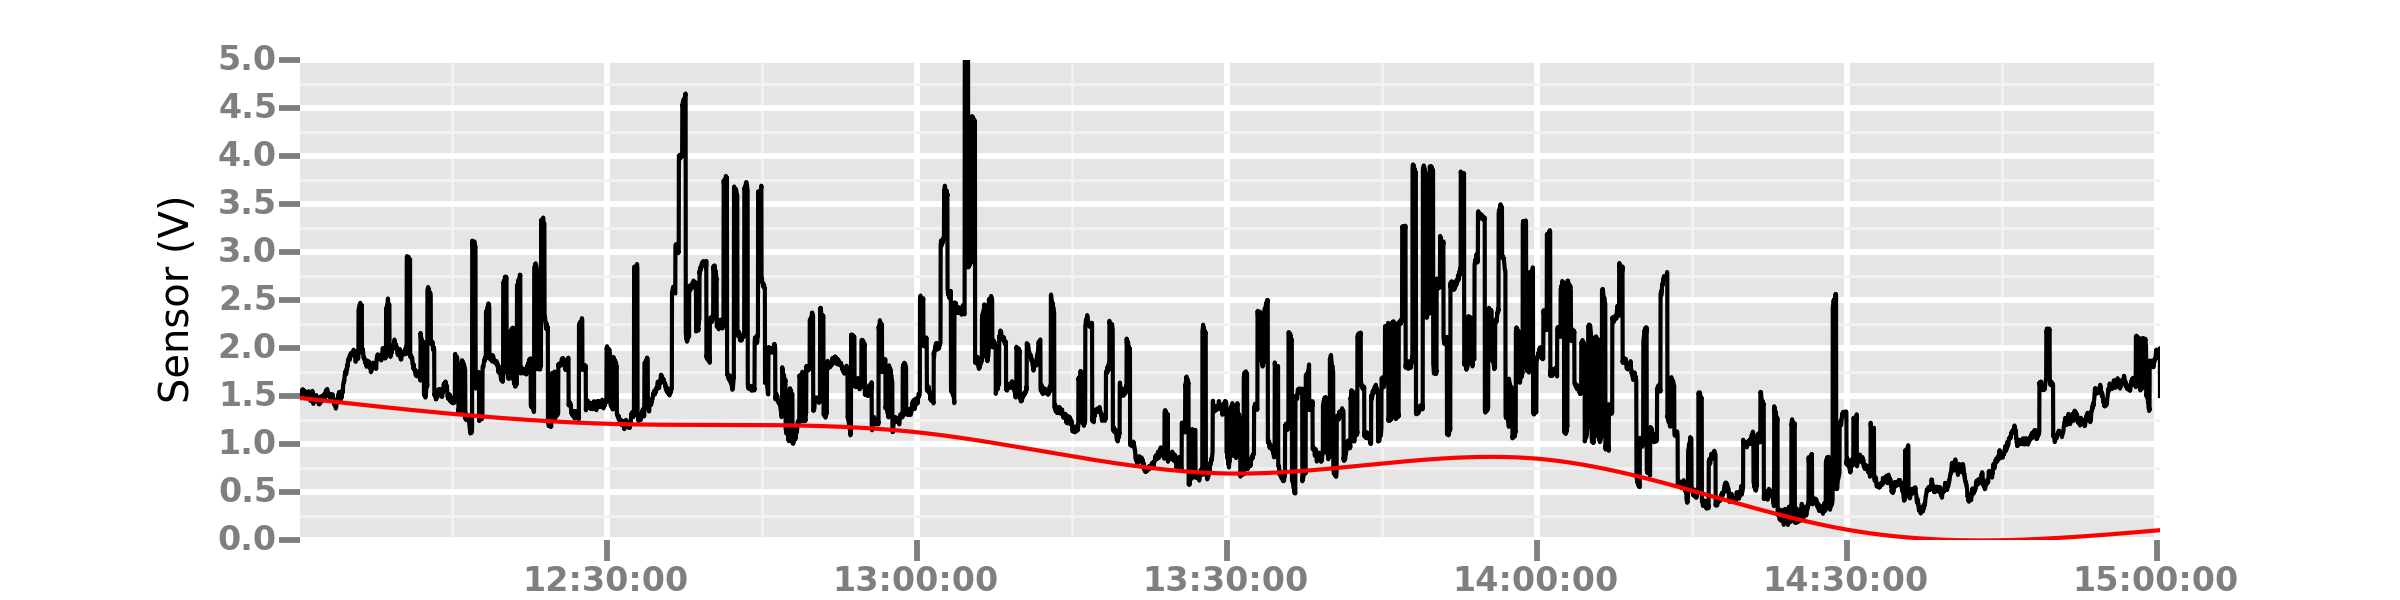
\includegraphics[width=\linewidth]{Spline_fit}
	\captionof{figure}{Example of baseline fit using Quantile Regression}
\end{center}


\subsection{Butterworth Bandpass Filter} 
The second method used to separate out the concentration signal was based on differences in frequency. The measured (and simulated) data consists of a low frequency baseline drift component, a high-frequency noise component and the concentration signal which appears to occur at a frequency in between the drift and the noise. 

The Butterworth bandpass filter is an infinite impulse response (IIR) filter. Given an imput signal $X(n)$ and an output signal $Y(n)$ the difference equation for an IIR filter is
$$ \sum_{j=0}^Q a_jy[n-j] = \sum_{i=0}^Pb_ix[n-i]$$
The transfer function of the filter is based on the frequency domain, so a Laplace-transform is used to convert the signal from a time-domain $(n)$ to a frequency domain $(\omega)$. The IIR transfer function takes the form

$$ H(\omega) = \frac{Y(\omega)}{X(\omega)} = \frac{\sum_{i=0}^Pb_i\omega^{-i}}{\sum_{j=0}^Qa_j\omega^{-j}}$$

The Buttterworth filter is a maximally flat approximation to an ideal bandpass filter. The transfer function is given as
$$H(\omega) = \frac{1}{\sqrt{1+\left ( \frac{\omega}{\omega_c} \right ) ^{2n}}} = \frac{\sum_{i=0}^Pb_i\omega^{-i}}{\sum_{j=0}^Qa_j\omega^{-j}}$$

where, $n$ is the filter order and $\omega_c$ is the cutoff frequency. Estimates for $\mathbf{a}$ and $\mathbf{b}$ were obtained using the \texttt{butter} function in the Scipy Signal Processing module with a frequency window of (0.01, 0.1) and order 2. Several different frequency were tested, and the window chosen resulted in the least visible drift and most signal. The filter was applied using the \texttt{filtfilt} function.   After the filter was applied the voltage was converted into a boolean variable with 1 sec values above 0.08 set to 1. 
\begin{center}			
	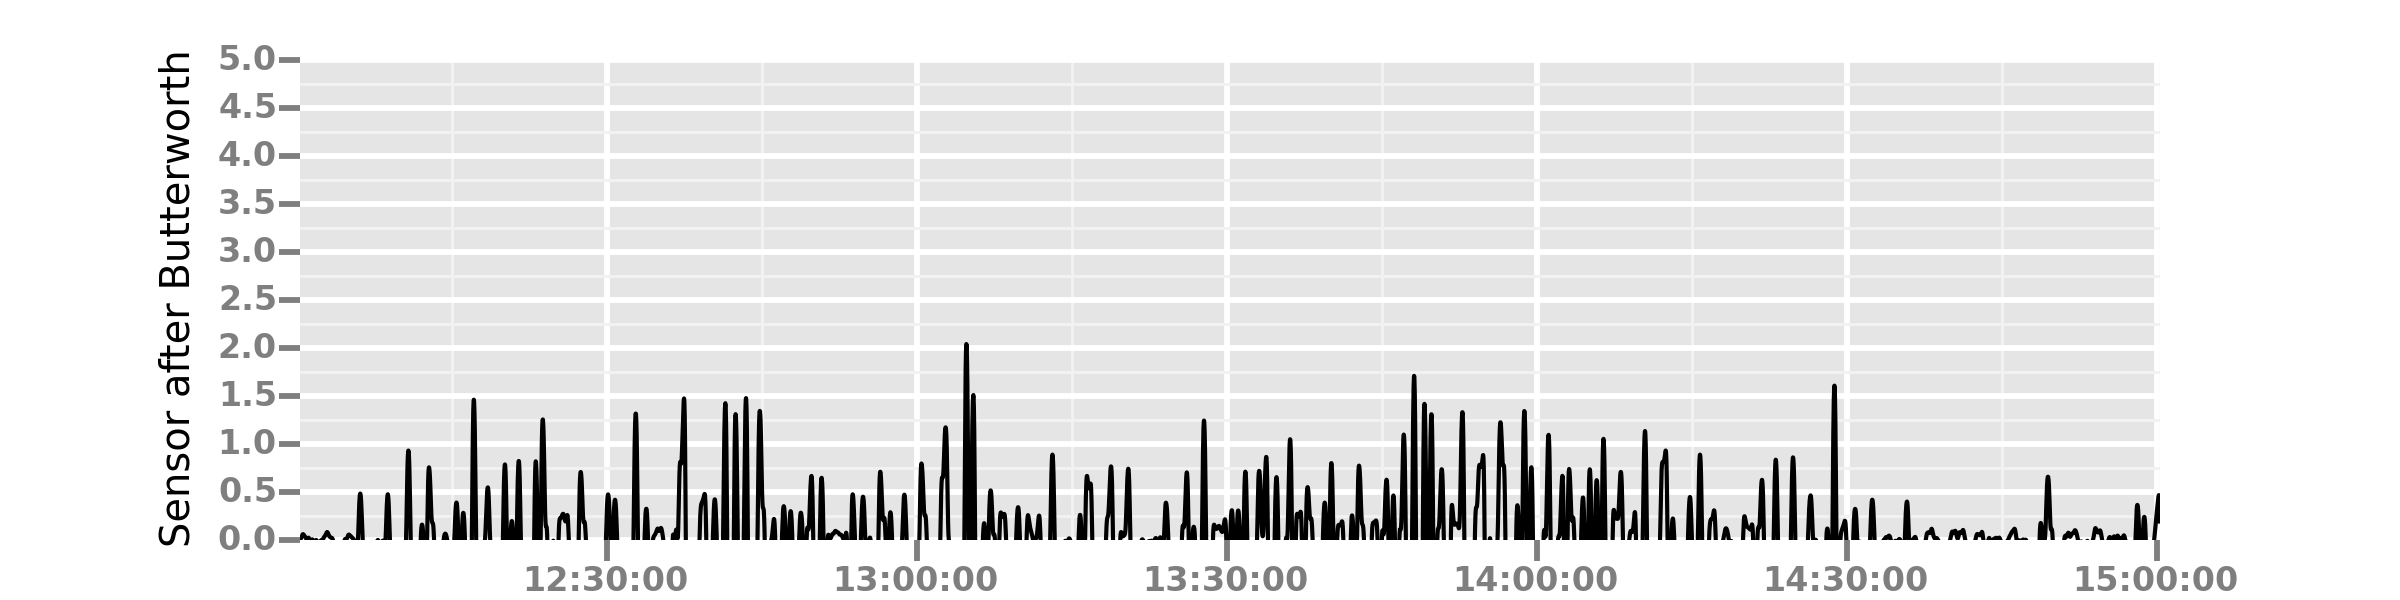
\includegraphics[width=\linewidth]{Butterworth_filt}
	\captionof{figure}{Example of sensor data after applying the bandpass filter}
\end{center}

\newpage


\section{Results}
\subsection{Simulated Data} 

	
True signal was defined as a boolean variable with value 1 if the 1 sec simulated signal was greater than 0.1 V, and 0 otherwise. Each five minute interval was categorized as "signal present" if signal was present for more than 5 sec within the interval, i.e mean value of the true signal was greater than 5/300. 
Both the bandpass filter method and the quantile regression method were able to correctly identify 65\% of the 5 min periods with true signal. The bandpass filter method had false positive rate of 10\% while the quantile regression method had a false positive rate of 20\%.   

\begin{figure}[h!]
	\centering			
	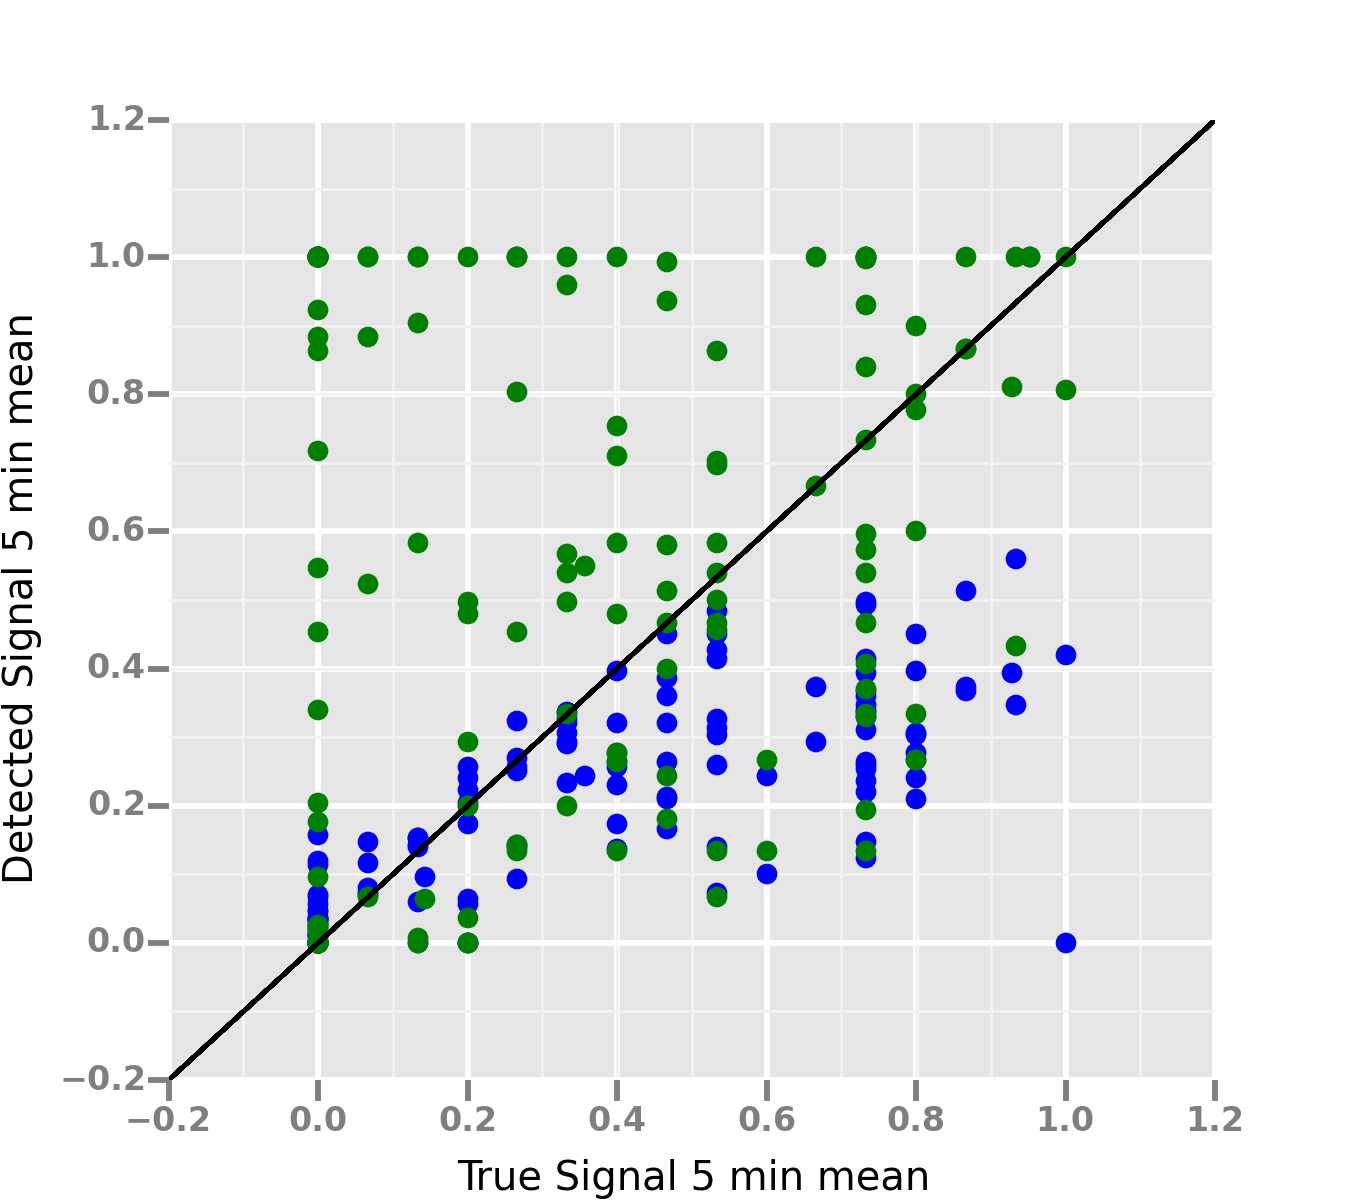
\includegraphics[width=0.4\linewidth]{TrueVDetect}
	\captionof{figure}{True versus detected signal, green represents quantile regression and blue represents the bandpass filter. Values are 5 min means of 1 sec boolean signal variables.}
\end{figure}

\subsection{Application}
The bandpass filter algorithm was applied to the sensor data from 11/1/14 to 11/30/14. The resulting 5 min filtered and averaged data set was divided into three categories: (1) time periods when signal was detected at the base sensor, (2) time periods when signal was detected at the SPod sensor, and (3) time periods when no signal was detected. The windroses below show the distribution of 5 min wind vectors in each of the categories. The wind vectors point to a single source emissions northeast of the sensors. The source is likely intermittent since there were periods of time when the wind blew from the north east and no signal was observed. 

\begin{figure}[h!]
	\begin{subfigure}[b]{0.3\textwidth}
		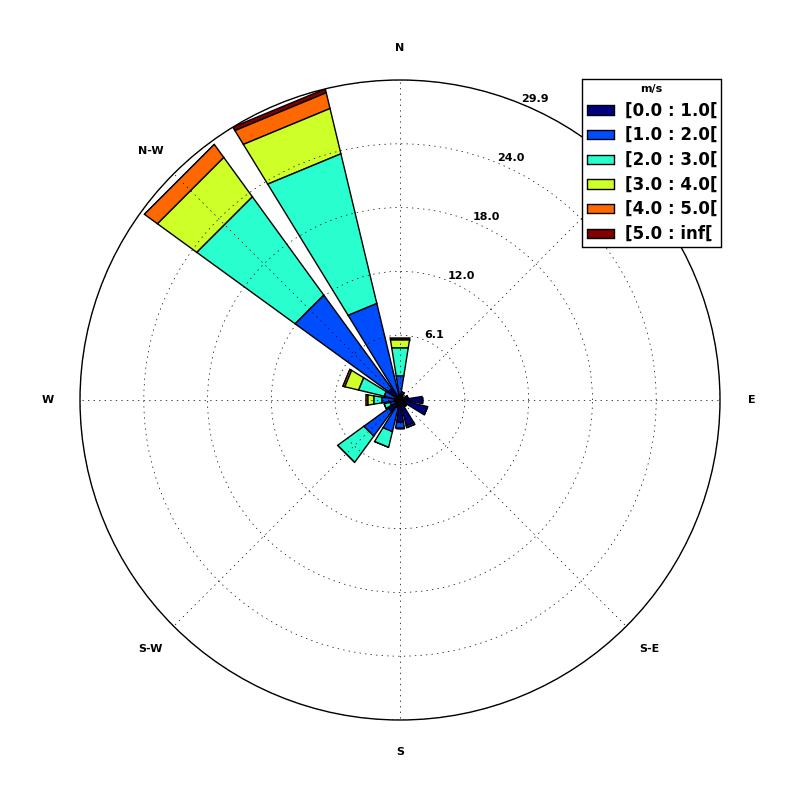
\includegraphics[width=\linewidth]{windrose_Base}
		\captionof{figure}{Signal at the Base.}
	\end{subfigure}
	\begin{subfigure}[b]{0.3\textwidth}			
		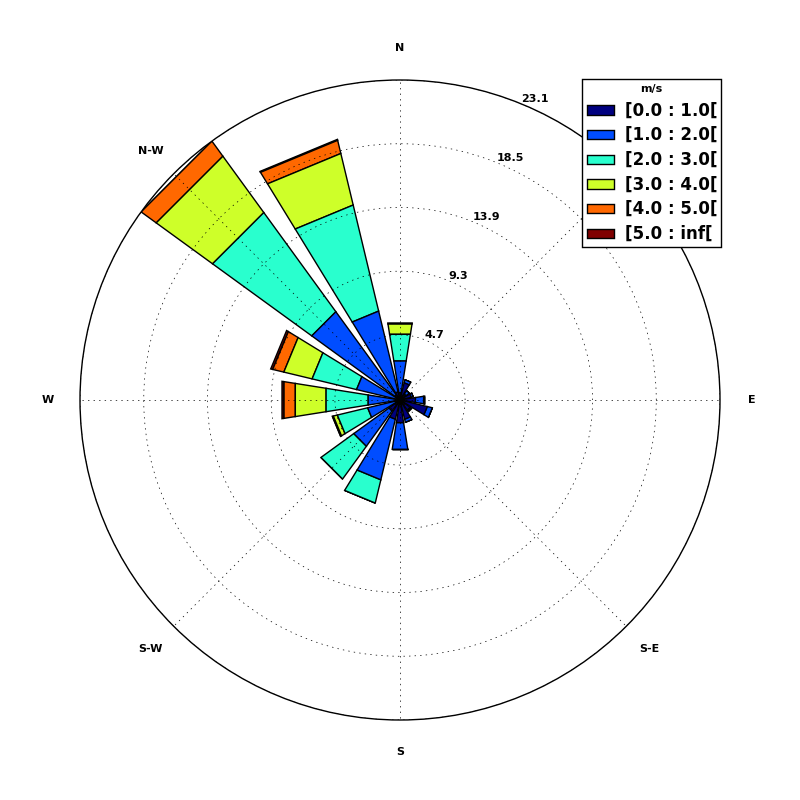
\includegraphics[width=\linewidth]{windrose_Remote}
		\captionof{figure}{Signal at the SPod.}
	\end{subfigure}
	\begin{subfigure}[b]{0.3\textwidth}		
		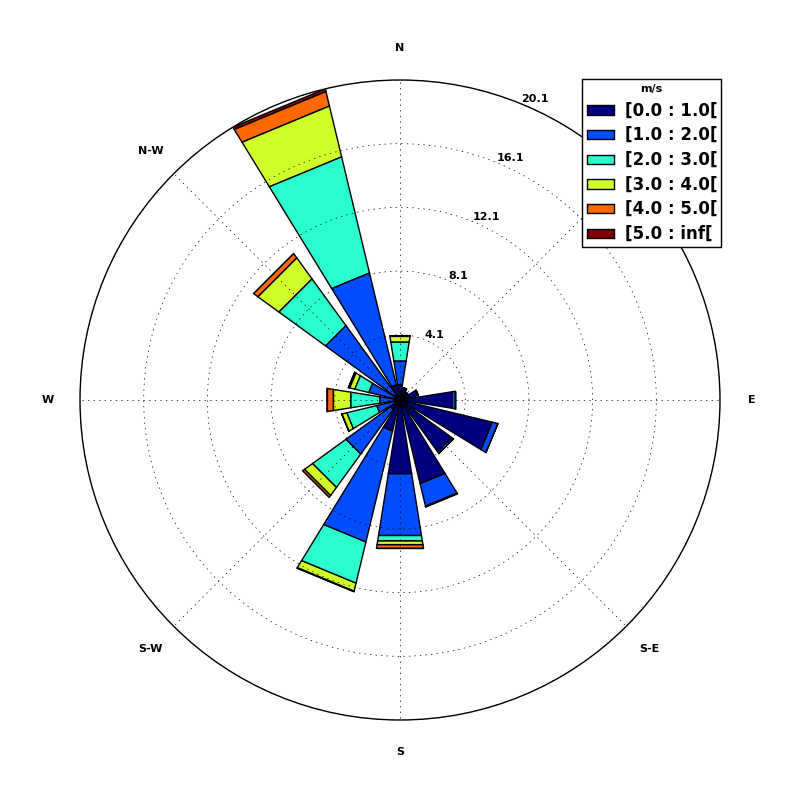
\includegraphics[width=\linewidth]{windrose_None}
		\captionof{figure}{No signal detected.}
	\end{subfigure}
\end{figure}

\newpage 

\bibliographystyle{abbrv}
\bibliography{references}

\newpage
\section{Appendix}
The python code and example data for this project  are contained in "leakDetection.zip". \\
Data files: \\   
Simulated\_07052014\_5min.csv - the simulated concentration dataset from the QUIC dispersion model.\\ 
SENTINEL Data\_2014-07-05.csv - example sensor file\\
SENTINEL Data\_2014-11-14.csv - example sensor file\\
Code files: \\
SPOD\_functions.py - contains the function definitions for both the algorithm and simulation.\\
Simulate\_Data.py - produces the simulated dataset and corresponding results\\
SPOD\_algorithm.py - applys the algorithm to the sensor data.
\end{document}